% ====================================================================
% BAB 2: TINJAUAN PUSTAKA
% ====================================================================
% File ini berisi tinjauan pustaka yang mencakup:
% - Penelitian terdahulu yang relevan
% - Landasan teori
% - Kerangka konseptual
%
% EDIT konten sesuai dengan penelitian Anda.
% ====================================================================

\chapter{TINJAUAN PUSTAKA}

% --- BAGIAN 2.1: PENELITIAN TERDAHULU ---
\section{Penelitian Terdahulu}
\label{sec:literature-related}

\begingroup
\pagestyle{fancy}
\singlespacing
\setlength{\extrarowheight}{4pt}
% \setlength{\LTleft}{-2cm}
% \setlength{\LTright}{-1cm}
\setlength{\LTpre}{-10pt}
\setlength{\LTpost}{1pt}

\begin{scriptsize}
	\begin{longtable}{>{\centering\arraybackslash}p{0.3cm} p{2.5cm} p{3cm} p{3cm} p{3cm}}

		\caption{Tinjauan Penelitian Terdahulu} \label{tab:tinjauan}                                                                                                                                                                                                                                                                                                                              \\[6pt]
		\hline
		\textbf{No}                                                                                                                                                                                                                                                                          & \textbf{Judul Penelitian} & \textbf{Hasil Penelitian} & \textbf{Celah (\textit{Gap})} & \textbf{Kontribusi} \\
		\hline
		\endfirsthead

		\caption*{\textbf{Tabel \ref{tab:tinjauan}} Tinjauan Penelitian Terdahulu}                                                                                                                                                                                                                                                                                                                \\[6pt]
		\hline
		\textbf{No}                                                                                                                                                                                                                                                                          & \textbf{Judul Penelitian} & \textbf{Hasil Penelitian} & \textbf{Celah (\textit{Gap})} & \textbf{Kontribusi} \\
		\hline
		\endhead

		\hline
		\endfoot

		\hline
		\endlastfoot

		1                                                                                                                                                                                                                                                                                    &
		\textit{A Topic Modeling Comparison Between LDA, NMF, Top2Vec, and BERTopic to Demystify Twitter Posts} \citep{10.3389/fsoc.2022.886498} (Jurnal Q1)                                                                                                                                 &
		Penelitian ini membandingkan BERTopic, NMF, LDA, dan Top2Vec pada data Twitter. BERTopic direkomendasikan untuk pendekatan berbasis \textit{embedding}, sedangkan NMF menjadi alternatif tradisional yang lebih unggul untuk data media sosial.                                      &
		Meskipun BERTopic menunjukkan performa yang baik, penggunaan \textit{embedding} multilingual dan \textit{clustering} default (HDBSCAN) masih memiliki keterbatasan dalam mengatasi \textit{outlier} dan meningkatkan stabilitas topik. Belum ada sistem aplikatif yang dikembangkan. &
		Penelitian ini menggunakan IndoBERTweet sebagai model \textit{embedding} khusus bahasa Indonesia serta BIRCH sebagai alternatif HDBSCAN untuk meningkatkan stabilitas \textit{clustering} dan mengurangi \textit{outlier}. Selain itu, dikembangkan sistem berbasis \textit{web} untuk analisis percakapan WhatsApp.                                                                      \\
		\hline
		2                                                                                                                                                                                                                                                                                    &
		\textit{Integrating IndoBERT and BIRCH in BERTopic for Indonesian short text} \citep{iaes2025indobert} (Jurnal Q2)                                                                                                                                                                   &
		Penelitian ini memodifikasi BERTopic dengan IndoBERT, BM25, dan BIRCH dengan dataset dari X,
		Google Reviews, dan YouTube yang bersifat teks monolog. Berhasil menurunkan \textit{outlier} secara signifikan serta meningkatkan stabilitas topik pada teks pendek.                                                                                                                 &
		Pendekatan ini belum dieksplorasi pada data percakapan grup WhatsApp yang memiliki karakteristik lebih kompleks berupa \textit{multi-turn dialogue}, evolusi percakapan yang cepat dan volume pesan yang tinggi.
		Selain itu, penelitian terdahulu belum menyediakan sistem aplikasi bagi pengguna akhir.                                                                                                                                                                                              &
		Penelitian ini mengimplementasikan BERTopic dengan IndoBERTweet
		dan BIRCH pada dataset WhatsApp yang diintegrasikan ke dalam sistem analisis
		interaktif untuk memvisualisasikan dinamika topik secara otomatis.                                                                                                                                                                                                                                                                                                                        \\
		\hline
		3                                                                                                                                                                                                                                                                                    &
		\textit{BERTopic Enhanced Bibliometric Insight Into Global South Higher Education} \citep{10643545} (Jurnal Q1)                                                                                                                                                                      &
		Penelitian ini menyelidiki keragaman linguistik dan proses dekolonisasi dalam sistem pendidikan tinggi di wilayah Global South menggunakan kerangka kerja empiris tiga tingkat yang menggabungkan Analisis Ko-okurensi Bibliometrik (Bibliometric Co-occurrence Analysis), pemodelan topik LDA, dan pemodelan BERTopic.
		BERTopic menunjukkan performa lebih baik dibanding LDA dalam koherensi dan jumlah topik yang dihasilkan pada data akademik.                                                                                                                                                          &
		Penelitian tersebut belum mengeksplorasi alternatif algoritma klasterisasi yang dapat meminimalkan \textit{outlier} sejak awal proses, serta belum menguji efektivitas BERTopic pada bahasa Indonesia dengan karakteristik teks percakapan informal yang memiliki noise tinggi dan fenomena \textit{code-mixing}.
		Penelitian tersebut juga belum menyediakan sistem aplikasi bagi pengguna akhir.                                                                                                                                                                                                                                         &
		Penelitian ini berkontribusi dengan
		mengganti HDBSCAN menggunakan BIRCH \textit{clustering} yang mampu mengakomodasi
		dokumen \textit{outlier} secara dinamis tanpa penghapusan, sekaligus menggunakan
		IndoBERTweet sebagai \textit{embedding} untuk dataset percakapan berbahasa Indonesia yang banyak mengandung kata informal dan \textit{code-mixing}.
		Penelitian ini juga menyediakan sistem aplikasi bagi pengguna akhir.                                                                                                                                                                                                                                                                                                                                                                                                                                                                                                           
		\\
	\end{longtable}
\end{scriptsize}
\setlength{\extrarowheight}{0pt}
\endgroup
% \newpage


Berdasarkan penelitian terdahulu yang telah diulas pada tabel \ref{tab:tinjauan}, dapat disimpulkan bahwa
meskipun telah banyak penelitian yang membandingkan berbagai model \textit{topic modeling} untuk analisis teks pendek, hasil penelitian terdahulu menunjukkan bahwa BERTopic cenderung lebih unggul dibandingkan pendekatan konvensional pada data media sosial dan data akademik, tetapi masih memiliki keterbatasan ketika menggunakan \textit{embedding} multilingual dan algoritma \textit{clustering} bawaan seperti HDBSCAN.
Pada sejumlah penelitian tersebut, penggunaan model yang lebih spesifik terhadap bahasa dan domain, seperti IndoBERT, serta algoritma BIRCH sebagai alternatif klasterisasi, terbukti menjanjikan dalam mengurangi \textit{outlier} dan meningkatkan stabilitas topik pada teks pendek.
Selain itu, penelitian yang telah diulas belum banyak mengeksplorasi penerapan pipeline BERTopic pada percakapan grup WhatsApp berbahasa Indonesia yang bersifat \textit{multi-turn}, tidak terstruktur, dan kaya \textit{code-mixing}. Di sisi lain, mayoritas penelitian masih berfokus pada evaluasi metodologi tanpa menyediakan sistem aplikasi yang dapat digunakan langsung oleh pengguna akhir untuk menganalisis percakapan mereka sendiri.

% --- BAGIAN 2.2: LANDASAN TEORI ---
\section{Landasan Teori}
\label{sec:literature-theory}

\subsection{Aplikasi WhatsApp}
\label{subsec:theory-first}

WhatsApp merupakan aplikasi pesan instan yang memungkinkan pengguna berkomunikasi melalui pesan teks, suara, gambar, video, serta fitur grup yang mendukung komunikasi banyak pengguna dalam satu ruang diskusi \citep{prayogi2025dinamika}.
Fitur grup memungkinkan pengguna tergabung dalam banyak kelompok sekaligus untuk kepentingan personal, bisnis, maupun keamanan, sehingga volume pesan sering menjadi besar dan tumpang tindih. Kondisi ini membuat percakapan grup bersifat tidak terstruktur, melibatkan banyak partisipan, dan topik pembahasan dapat berubah dengan cepat \citep{rani2022whatsapp}.
Akibatnya, pengguna sering kesulitan mengikuti arah percakapan secara menyeluruh. Permasalahan inilah yang menjadi latar belakang penelitian ini, yaitu mengembangkan sistem analisis percakapan grup WhatsApp yang dapat mengidentifikasi dan memetakan topik pembahasan secara otomatis.

\subsection{BERTopic}
\label{subsec:theory-second}

BERTopic adalah \textit{framework topic modeling} berbasis \textit{transformer}
yang membentuk \textit{embedding} dokumen dan merepresentasikan topik melalui
prosedur TF-IDF berbasis kelas, sehingga dokumen dengan makna semantik serupa
dapat dipetakan saling berdekatan dalam ruang vektor \citep{grootendorst2022bertopic}.
Pendekatan ini relevan untuk percakapan grup WhatsApp yang umumnya berupa teks
pendek, berisik (\textit{noisy}), dan tidak terstruktur, yang cenderung menimbulkan
masalah kelangkaan data (\textit{data sparsity}) pada metode pemodelan topik konvensional.

\begin{figure}[h]
	\centering
	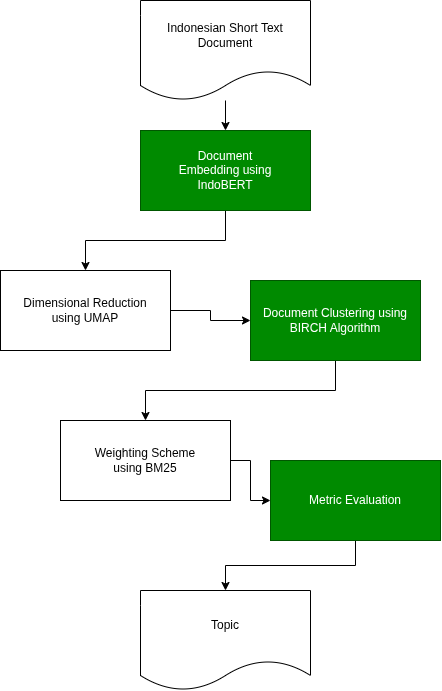
\includegraphics[width=0.45\textwidth]{images/framework-bertopic-modifikasi-indobert-birch-bm25.png}
	\caption{Framework BERTopic dengan modifikasi IndoBERT, BIRCH, dan BM25 \citep{iaes2025indobert}}
	\label{fig:framework-bertopic}
\end{figure}

Berdasarkan Gambar \ref{fig:framework-bertopic}, \textit{framework} BERTopic terdiri dari empat tahap utama. Tahap pertama adalah
\textit{document embedding} yang mengubah dokumen menjadi representasi vektor
numerik menggunakan model bahasa seperti IndoBERTweet yang dikembangkan untuk variasi bahasa Indonesia pada ranah media sosial \citep{koto2021indobertweet}. Tahap kedua adalah
\textit{dimensionality reduction} menggunakan UMAP untuk mereduksi dimensi vektor
hasil \textit{embedding} agar proses klasterisasi lebih efisien \citep{mcinnes2018umap}.
Tahap ketiga adalah \textit{clustering} yang mengelompokkan dokumen berdasarkan
kemiripan semantik, di mana setiap klaster merepresentasikan satu topik dengan
dukungan model yang bersifat modular seperti HDBSCAN, BIRCH, dan K-Means.
Tahap keempat adalah \textit{topic representation} yang mengekstrak kata kunci paling
representatif dari setiap klaster. Secara bawaan BERTopic menggunakan c-TF-IDF,
namun tahap ini dapat dimodifikasi karena bersifat modular \citep{grootendorst2022bertopic}.
Dalam penelitian ini, komponen yang digunakan pada tiap tahap meliputi IndoBERTweet
untuk \textit{embedding}, BIRCH untuk klasterisasi, dan BM25 untuk representasi topik.

% --- BAGIAN 2.3: KERANGKA KONSEPTUAL (OPSIONAL) ---
\subsection{IndoBERTweet}
\label{subsec:indobertweet}

Model IndoBERTweet merupakan model bahasa pra-latih berskala besar pertama yang dirancang khusus untuk memproses data Twitter (X) berbahasa Indonesia.
Model ini dikembangkan melalui pendekatan \textit{domain-adaptive pretraining} dengan fondasi IndoBERT yang semula dilatih pada korpus formal, kemudian diadaptasi ke domain Twitter yang lebih informal.
Dalam proses adaptasi tersebut, peneliti melakukan penyesuaian kosakata domain-spesifik dan melaporkan 14.584 kosakata baru (46\% dari total kosakata) yang tidak tercakup pada IndoBERT umum \citep{koto2021indobertweet}.

\begingroup
\pagestyle{fancy}
\renewcommand{\arraystretch}{1}
\begin{table}[H]
	\centering
	\caption{Perbandingan Kinerja Model pada Tujuh Tugas}\label{tab:kinerja-indobertweet}
	\setlength{\tabcolsep}{4pt}
	\scriptsize
	\begin{tabular}{>{\arraybackslash}p{3.8cm}ccccccc>{\centering\arraybackslash}p{1.5cm}}
		\toprule
		\multirow{2}{*}{{\textbf{Model}}}                                          & \multicolumn{2}{c}{\textbf{Sentiment}} & \textbf{Emotion} & \multicolumn{2}{c}{\textbf{Hate Speech}} & \multicolumn{2}{c}{\textbf{NER}} & \multirow{2}{*}{\parbox{2cm}{\textbf{Average}}}                                                       \\
		\cmidrule(lr){2-3}\cmidrule(lr){4-4}\cmidrule(lr){5-6}\cmidrule(lr){7-8}
		                                                                           & \textbf{IndoLEM}                       & \textbf{SmSA}    & \textbf{EmoT}                            & \textbf{HS1}                     & \textbf{HS2}                                    & \textbf{Formal} & \textbf{Informal} &               \\
		\midrule
		mBERT                                                                      & 76.6                                   & 84.7             & 67.5                                     & 85.1                             & 75.1                                            & 85.2            & 83.2              & 79.6          \\
		malayBERT                                                                  & 82.0                                   & 84.1             & 74.2                                     & 85.0                             & 81.9                                            & 81.9            & 81.3              & 81.5          \\
		IndoBERT \citep{wilie2020indonlu}                                          & 84.1                                   & 88.7             & 73.3                                     & 86.8                             & 80.4                                            & 86.3            & 84.3              & 83.4          \\
		IndoBERT \citep{Indobert2020}                                              & 84.1                                   & 87.9             & 71.0                                     & 86.4                             & 79.3                                            & 88.0            & 86.9              & 83.4          \\
		IndoBERTweet (1M steps from scratch) \citep{koto2021indobertweet}          & 86.2                                   & 90.4             & 76.0                                     & \textbf{88.8}                    & \textbf{87.5}                                   & \textbf{88.1}   & 85.4              & 86.1          \\
		IndoBERT + Vocabulary adaptation + 200K steps \citep{koto2021indobertweet} & \textbf{86.6}                          & \textbf{92.7}    & \textbf{79.0}                            & 88.4                             & 84.0                                            & 87.7            & \textbf{86.9}     & \textbf{86.5} \\
		\bottomrule
	\end{tabular}
\end{table}
\endgroup


Berdasarkan Tabel \ref{tab:kinerja-indobertweet} yang diadaptasi dari \cite{koto2021indobertweet}, model IndoBERTweet dan variannya subsecara konsisten mencapai performa tinggi pada tujuh tugas NLP berbahasa Indonesia, meliputi \textit{sentiment analysis}, \textit{emotion classification}, \textit{hate speech detection}, dan \textit{named entity recognition}.
Hasil terbaik secara rata-rata ditunjukkan oleh varian IndoBERT dengan adaptasi kosakata dan pelatihan lanjutan 200K langkah (86{,}5), sedangkan IndoBERTweet yang dilatih dari awal juga menunjukkan kinerja kompetitif (86{,}1).
Temuan ini memperkuat asumsi bahwa model berbasis domain media sosial berpotensi lebih sesuai untuk teks pendek, informal, dan bising seperti percakapan grup WhatsApp berbahasa Indonesia, meskipun efektivitas akhirnya tetap perlu divalidasi pada penelitian ini.


\subsection{BIRCH Clustering}
\label{subsec:birch}

BIRCH (\textit{Balanced Iterative Reducing and Clustering using Hierarchies}) merupakan algoritma \textit{clustering}
hierarkis yang dirancang untuk menangani dataset berskala besar secara efisien dengan cara meringkas data ke dalam
struktur \textit{Clustering Feature} (CF) yang disusun dalam CF-Tree di memori, sehingga mengurangi kebutuhan komputasi
dibandingkan pendekatan yang memproses setiap titik data secara individual \citep{10.1145/235968.233324}.
Algoritma ini memiliki keunggulan dalam efisiensi komputasi, penggunaan memori yang rendah, serta ketahanan
terhadap \textit{noise}, namun tetap memiliki keterbatasan, seperti sensitivitas terhadap parameter \textit{threshold},
kesulitan dalam menangani klaster dengan bentuk kompleks, serta kurang optimal pada dataset berdimensi tinggi \citep{10.1023/A:1009783824328}.
Dalam konteks framework BERTopic, keterbatasan terkait dimensi tinggi tersebut dapat diminimalkan melalui
penerapan UMAP sebagai teknik reduksi dimensi sebelum proses klasterisasi dilakukan.

Pada implementasi BIRCH di \textit{scikit-learn}, ringkasan tiap subklaster disimpan
dalam bentuk \textit{Clustering Feature} (CF) sebagaimana didefinisikan pada BIRCH
orisinil dan dipaparkan kembali pada kajian implementasi matematis modern
\citep{10.1145/235968.233324,IJECE25896}:

\begin{equation}
	CF = (N, LS, SS)
\end{equation}

\noindent dengan $N$ jumlah titik data, $LS = \sum_{i=1}^{N} x_i$, dan
$SS = \sum_{i=1}^{N} \lVert x_i \rVert^2$.

Centroid subklaster dihitung sebagai:

\begin{equation}
	\mu = \frac{LS}{N}
\end{equation}

Radius subklaster digunakan sebagai dasar keputusan pemisahan/penggabungan node.
Bentuk komputasional berikut ekuivalen dengan definisi radius BIRCH
\citep{10.1145/235968.233324,IJECE25896}:

\begin{equation}
	R = \sqrt{\frac{SS}{N} - \left\lVert \frac{LS}{N} \right\rVert^2}
\end{equation}

Ketika titik baru $x$ ditambahkan ke subklaster, radius baru dihitung menggunakan
prinsip aditivitas CF, lalu dibandingkan dengan \textit{threshold} ($T$)
\citep{10.1145/235968.233324,IJECE25896}:

\begin{equation}
	R' = \sqrt{\frac{SS + \lVert x \rVert^2}{N+1} - \left\lVert \frac{LS + x}{N+1} \right\rVert^2}, \quad R' \le T
\end{equation}

Parameter \textit{branching factor} ($B$) mengontrol jumlah maksimum anak pada tiap
node CF-Tree, sedangkan $T$ mengontrol kekompakan subklaster.


\subsection{Topic Representation Dengan BM25}
\label{sec:bm25}

% TODO: Revisi menambahkan penjelasan mengenai kenapa kok BM25 ini dipakai pada penelitian ini
    Skema pembobotan BM25 adalah algoritma fungsi peringkat (ranking function) yang banyak digunakan dalam pencarian informasi (information retrieval) dan dapat diadaptasi untuk tahap representasi topik \citep{doi.org/10.1111/coin.12248,DBLP:journals/corr/abs-2007-05186}. 
	c-TF-IDF kesulitan menangkap hubungan semantik secara utuh dan cenderung menghasilkan topik yang kurang koheren ketika distribusi frekuensi kata sangat timpang atau tidak merata \citep{iaes2025indobert}. Oleh karena itu, sejumlah
penelitian menerapkan BM25 pada tahap \textit{topic representation}, baik sebagai
pengganti penuh maupun sebagai modifikasi dari skema c-TF-IDF.

Pada penelitian \citep{iaes2025indobert}, c-TF-IDF bawaan BERTopic digantikan
sepenuhnya dengan BM25 pada level klaster, dengan skor kata dirumuskan sebagai:
\begin{equation}
	w_{t,c_k} = \sum_{d \in C_k} IDF(t) \cdot
	\frac{f(t,d)(k_1 + 1)}
	{f(t,d) + k_1 \left(1 - b + b \cdot \frac{|d|}{avgdl}\right)},
\end{equation}
dengan fungsi \textit{inverse document frequency} didefinisikan sebagai
$IDF(t) = \log \left( \frac{N - n(t) + 0.5}{n(t) + 0.5} \right)$.
Skor $w_{t,c_k}$ pada persamaan tersebut dihitung dengan menjumlahkan kontribusi
seluruh dokumen $d$ yang menjadi anggota himpunan dokumen pada klaster ke-$k$,
yang dinotasikan sebagai $C_k$. Untuk setiap dokumen tersebut, $f(t,d)$
menyatakan frekuensi kemunculan kata $t$ di dalam dokumen $d$, sementara $|d|$
menyatakan panjang dokumen $d$ yang kemudian dinormalisasi terhadap $avgdl$,
yaitu rata-rata panjang dokumen dalam korpus. Adapun nilai $IDF(t)$ diperoleh
dari $n(t)$, yang menyatakan jumlah dokumen dalam korpus yang memuat kata $t$,
serta $N$ yang menyatakan jumlah total dokumen dalam korpus tersebut. Dua
parameter tambahan, $k_1$ dan $b$, masing-masing berfungsi mengatur tingkat
saturasi frekuensi istilah agar pengaruh kata yang berulang tidak meningkat
secara linear, dan mengatur normalisasi panjang dokumen agar dokumen yang
lebih panjang tidak secara otomatis memperoleh skor yang lebih tinggi.

Dalam konteks studi tersebut, pendekatan ini dilaporkan memberikan representasi
topik yang lebih stabil dibandingkan c-TF-IDF pada korpus teks pendek berbahasa
Indonesia \citep{iaes2025indobert}.

\subsection{Topic Coherence}
\label{subsec:topic-coherence}

\textit{Topic coherence} digunakan untuk mengukur keterkaitan semantik antar kata teratas dalam topik. Dari banyaknya \textit{topic coherence}, penelitian ini menggunakan \textit{Normalized Pointwise Mutual Information} (NPMI) karena memberikan korelasi tertinggi dengan penilaian manusia dalam konteks context vectors \citep{2685324}:

\begin{equation}
    \text{NPMI}(w_i, w_j) = 
    \frac{
        \log \dfrac{P(w_i, w_j)}{P(w_i) \cdot P(w_j)}
    }{
        -\log P(w_i, w_j)
    }
    \label{eq:npmi-standalone}
\end{equation}

\noindent dengan $P(w_i,w_j)$ sebagai probabilitas ko-okurensi, serta $P(w_i)$ dan $P(w_j)$ sebagai probabilitas
marjinal kemunculan kata. Nilai dari NPMI berkisar antara [-1, 1], dengan nilai 1 menunjukkan keterkaitan semantik yang sempurna, 0 menunjukkan tidak ada keterkaitan, dan nilai negatif menunjukkan keterkaitan yang berlawanan \citep{11271424}.

\subsection{Topic Diversity}
\label{subsec:topic-diversity}

\textit{Topic diversity} didefinisikan dengan keberagaman topik sebagai persentase kata unik dalam 25 kata teratas dari semua topik. Keberagaman mendekati 0 menunjukan bahwa topik yang berlebihan dan keberagaman mendekati 1 menunjukkan topik yang beragam \citep{dieng2020topic}. Nilainya dihitung
melalui rumus berikut:

\begin{equation}
	TD = \frac{|\text{unique words in top } N \text{ words of all topics}|}{N \times K}
\end{equation}

\subsection{Embedding Density}
\label{subsec:embedding-density}

\textit{Embedding Density} adalah metrik evaluasi yang mengukur tingkat kekompakan (\textit{compactness}) representasi embedding dokumen di dalam suatu klaster atau topik \citep{2009-00672}. Metrik ini dihitung menggunakan fungsi kernel dengan bobot sebagai berikut:

\begin{equation}
\rho_k(z) =
\frac{
\sum_{i=1}^{N_k} K\!\left(\dfrac{z - \mathbf{e}_i^{(k)}}{h}\right) w_{k,i}
}{
\sum_{i=1}^{N_k} K\!\left(\dfrac{z - \mathbf{e}_i^{(k)}}{h}\right)
}
\label{eq:embedding-density}
\end{equation}

\noindent dengan $z$ adalah titik embedding evaluasi, yang dalam
penelitian ini ditetapkan sebagai centroid embedding topik $k$
($z = \bar{\mathbf{e}}^{(k)}$); $\mathbf{e}_i^{(k)}$ adalah vektor
embedding dokumen ke-$i$ dalam topik $k$; $N_k$ adalah jumlah dokumen
dalam topik $k$; $K(\cdot)$ adalah fungsi kernel Gaussian; $h$ adalah
parameter \textit{bandwidth}; dan $w_{k,i}$ adalah bobot representativitas
dokumen ke-$i$ terhadap topik $k$, yang dihitung berdasarkan
\textit{cosine similarity} antara embedding dokumen dan centroid
embedding topik tersebut. Semakin tinggi nilai kepadatan yang diperoleh, semakin kohesif dan bermakna topik yang dihasilkan \citep{2009-00672}.

\subsection{Intra-topic Similarity}
\label{subsec:intra-topic-similarity}

Intra-topic similarity merupakan metrik evaluasi yang mengukur kemiripan 
semantik antar dokumen di dalam satu topik, diadaptasi dari konsep 
\textit{intra-list similarity} (ILS) sebagai rata-rata kemiripan berpasangan 
seluruh item dalam sebuah daftar \citep{10.1007/s11257-022-09351-w}. \cite{zhao2018inter} menekankan bahwa struktur intra-topik berbasis 
\textit{word embeddings} mampu menangkap aspek tematik yang lebih halus dan 
bermakna. Dalam konteks evaluasi model topik, intra-topic similarity untuk 
topik $k$ dengan $N_k$ dokumen dirumuskan sebagai berikut:
\begin{equation}
    \text{ITS}(k) = \frac{1}{N_k(N_k - 1)} 
        \sum_{\substack{i,j=1 \\ i \neq j}}^{N_k}
        \cos\!\left(\mathbf{e}_i^{(k)},\, \mathbf{e}_j^{(k)}\right)
    \label{eq:intra-topic-similarity}
\end{equation}

\noindent di mana $\mathbf{e}_i^{(k)}$ dan $\mathbf{e}_j^{(k)}$ adalah 
embedding dokumen ke-$i$ dan ke-$j$ dalam topik $k$. Nilai akhir diperoleh 
dengan merata-ratakan $\text{ITS}(k)$ di seluruh $K$ topik; semakin tinggi 
nilainya, semakin kohesif topik yang dihasilkan.

% Gunakan diagram jika tersedia (lihat contoh di bawah):
% \begin{figure}[h]
% \centering
% \includegraphics{images/conceptual-framework.png}
% \caption{Kerangka Konseptual Penelitian}
% \label{fig:framework}
% \end{figure}

% ====================================================================
% CATATAN PENGISIAN BAB TINJAUAN PUSTAKA:
%
% 1. PENELITIAN TERDAHULU:
%    - Minimal 10 referensi (sesuai juknis)
%    - Urutkan secara kronologis atau tematik
%    - Highlight gap/celah yang akan Anda isi
%    - Cite dengan benar (gunakan Mendeley/Zotero)
%
% 2. LANDASAN TEORI:
%    - Jelaskan teori relevan (2-4 teori utama)
%    - Gunakan subsection untuk mengorganisir
%    - Berikan konteks dan aplikasi praktis dari teori
%    - Jangan hanya copy-paste, jelaskan dengan kata-kata Anda
%
% 3. KERANGKA KONSEPTUAL:
%    - Hubungkan teori dengan penelitian Anda
%    - Jelaskan variabel independen, dependen, kontrol (jika ada)
%    - Bisa dalam bentuk deskripsi atau diagram
%    - Ini adalah "jembatan" antara teori dan metodologi
%
% 4. SITASI:
%    - Gunakan format APA (sesuai juknis)
%    - Minimal 50% referensi dari 10 tahun terakhir
%    - Tambah file references.bib untuk bibliography
% ====================================================================
